\chapter{Architectural description}

\section{Architecure}

\subsection{Architectural viewport selection}
The “4+1 view model” \cite{bib:vm} by Philippe Kruchten suggest four different view, logical, process, development and physical. In the case of XOXOmail we are going to use the logical, process and development view. The rationale behind removing the physical view is that XOXOmail will run on a single physical device and only utilize one process, a security view, describing the layers of security, will be added instead.

\subsection{Logical view (Object oriented deomposition)}
“The logical architecture primarily supports the functional requirements --- what the system should provide in terms of services to its users. The system is decomposed into a set of key abstractions, taken from the problem domain, in the form of objects or object classes” \cite{bib:vm}. A common way to represent this view is with a class diagram that shows a set of classes and their relationships. As you can see, we have chosen to divide the logical view into three parts: GUI, Service and Model. 
See figure \ref{fig:logicalview} at page \pageref{fig:logicalview}.

\subsubsection{GUI}
The GUI represents the Android frontend, which is made up of activities. This is what the user actually sees. All the activities extends WrapperActivity, which is the GUI connection to the service part of our app.

\subsubsection{Service}
 This is what holds the main logic of the app and all services are available from the ServiceProvider. Hardware abstraction layer (HAL), Persistence, Security and Network is available from here. 

\subsubsection{Model}
Here you will find all classes that wrap information that is needed throughout the app. The models include objects for current user, for the XOMessage which holds the message itself and all its attributes. And of course we also have all of the settings for our app here, just to name a few. 

\begin{figure}
	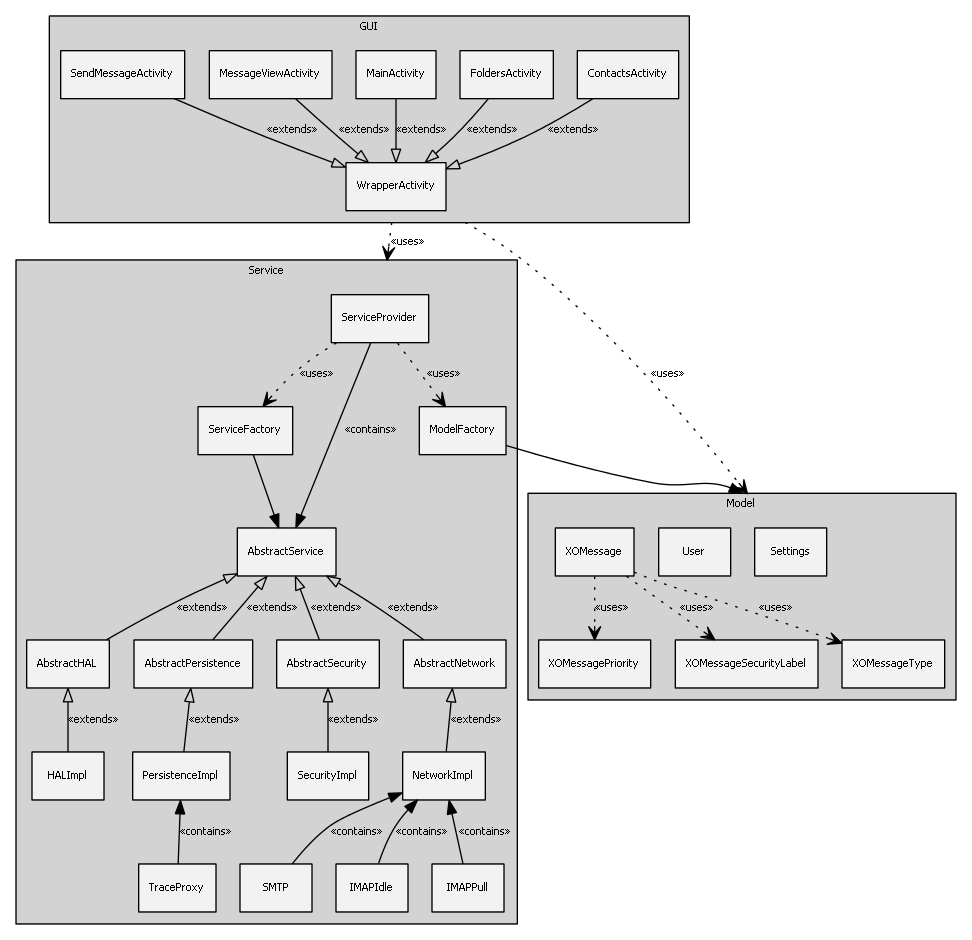
\includegraphics[width=\textwidth]{logicalview.png}
	\caption{The logical view of the architecture}
	\label{fig:logicalview}
\end{figure}

\subsection{Development view (Subsystem decomposition)}
The development view is a step up from the logical view and focuses on software modules instead of classes. These subsystems/modules are organized in a hierarchy of layers where each layer provides a well-defined interface to layers above. “The complete development architecture can only be described when all the elements of the software have been identified. It is, however, possible to list the rules that govern the development architecture: partitioning, grouping, visibility" \cite{bib:vm}. 
See figure \ref{fig:developmentview} at page \pageref{fig:developmentview}. As you can see, the Backend Service Connects to all parts of our app. The main focus of this view is to show that it is also the connector to the external part of the app, the SMTP Gateway. This gateway is implemented by Thales, and all we have to do is connect to it using well known protocols.

\begin{figure}
	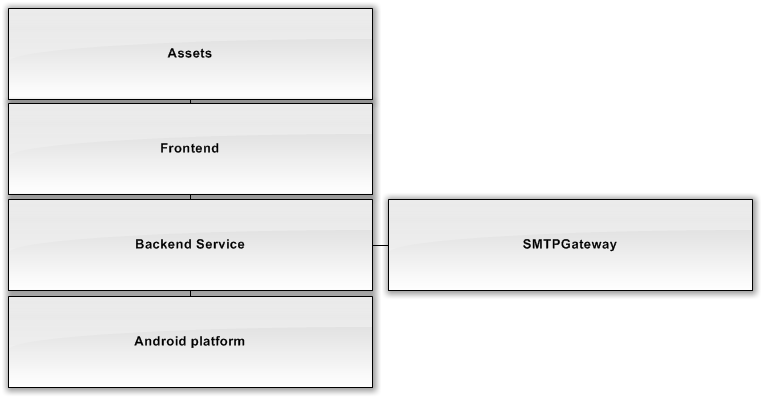
\includegraphics[width=\textwidth]{developmentview.png}
	\caption{Development View}
	\label{fig:developmentview}
\end{figure}

\subsection{Process View}
The process view is concerned with how different tasks bind together to form one executable unit. More specifically, the communication between threads/processes and on which thread/process is a task executed. We will differentiate between major and minor tasks, where major tasks are architectural elements open through a public interface, and minor tasks being tasks introduced in order to implement some functionality in one class or module.  
See figure \ref{fig:processview} at page \pageref{fig:processview}. As an example, you can here see that IMAPThread og IMAPIdleThread are minor tasks, because theay are just tasks that need to be implemented for making a bigger functionality work, namely the ServiceProvider.

\begin{figure}
	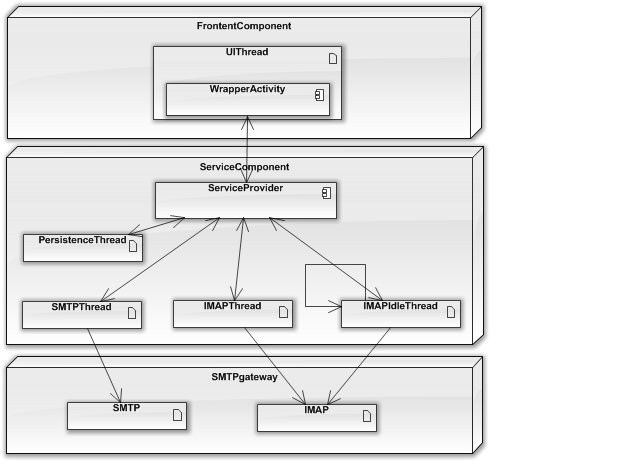
\includegraphics[width=\textwidth]{processview.png}
	\caption{Process view}
	\label{fig:processview}
\end{figure}

\subsection{Security View}
The security view is concerned with how the system as a whole is secured. This involves intercommunication, storage and communication with external sources. The view is not however concerned about implementation, just the layers of security.
See figure \ref{fig:securityview} at page \pageref{fig:securityview}.

\begin{figure}
	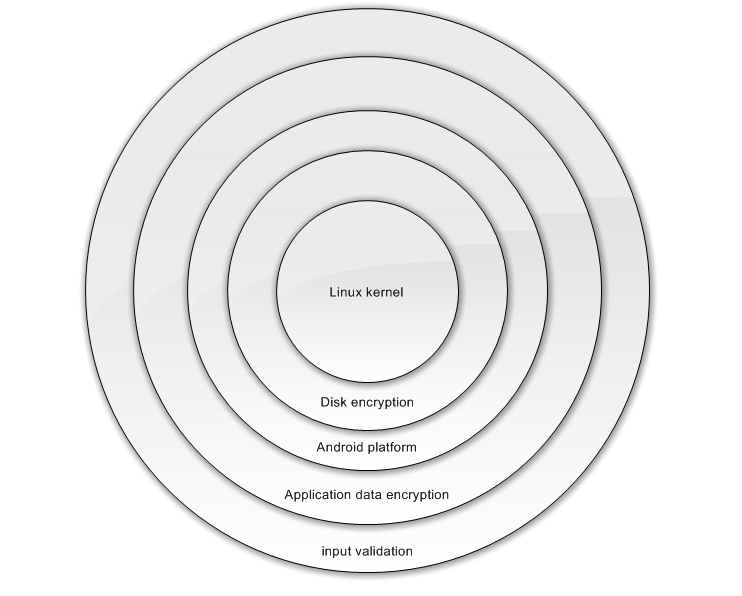
\includegraphics[width=\textwidth]{securityview.png}
	\caption{Security view}
	\label{fig:securityview}
\end{figure} \hfill
\newline
\newline
\textbf{The Linux kernel} provides us with a user-based permissions model and process isolation, which ensures that another process cannot access the memory of XOXOMail during runtime.
\newline
\newline
\textbf{Disk encryption}, is feature provided by the android platform, which encrypts the whole Android device using \gls{aes} with \gls{cbc} and \gls{essiv2}.\cite{bib:crypto}
\newline
\newline
\textbf{Android platform}, most of the security provided by the Android platform is provided by the Linux kernel, but not necessary used in normal conditions. The application sandbox is one of these things. And since the sandboxing operation is located at kernel level, it is hard to break out of. 
\newline
\newline
\textbf{Application data encryption} is a response to the possibility of rooted devices. Normally an android application will not run with root access on the device, this however is not the case on rooted devices. In which case the application and user will have full access to all applications and all application data. By adding our own encryption layer with the key stored off-device we can ensure data security even with root access to the phone\cite{bib:tech}. The encryption we opted for is an \gls{aes} based encryption with a user-password derived key by \gls{pbsha}.
Regarding communication with external resources as a mail-server, it will be done over a secure communication channel providing \gls{ssl1} or \gls{tls}. 
\newline
\newline
\textbf{Input validation} is always necessary in order to provide a secure service. All input to the XOXOMail application should be validated, this is includes received mail, user-input etc. For mail validation we are going to use \gls{emims} signing and verification provided by bouncycastle. 

\subsection{GUI}
\begin{figure}
	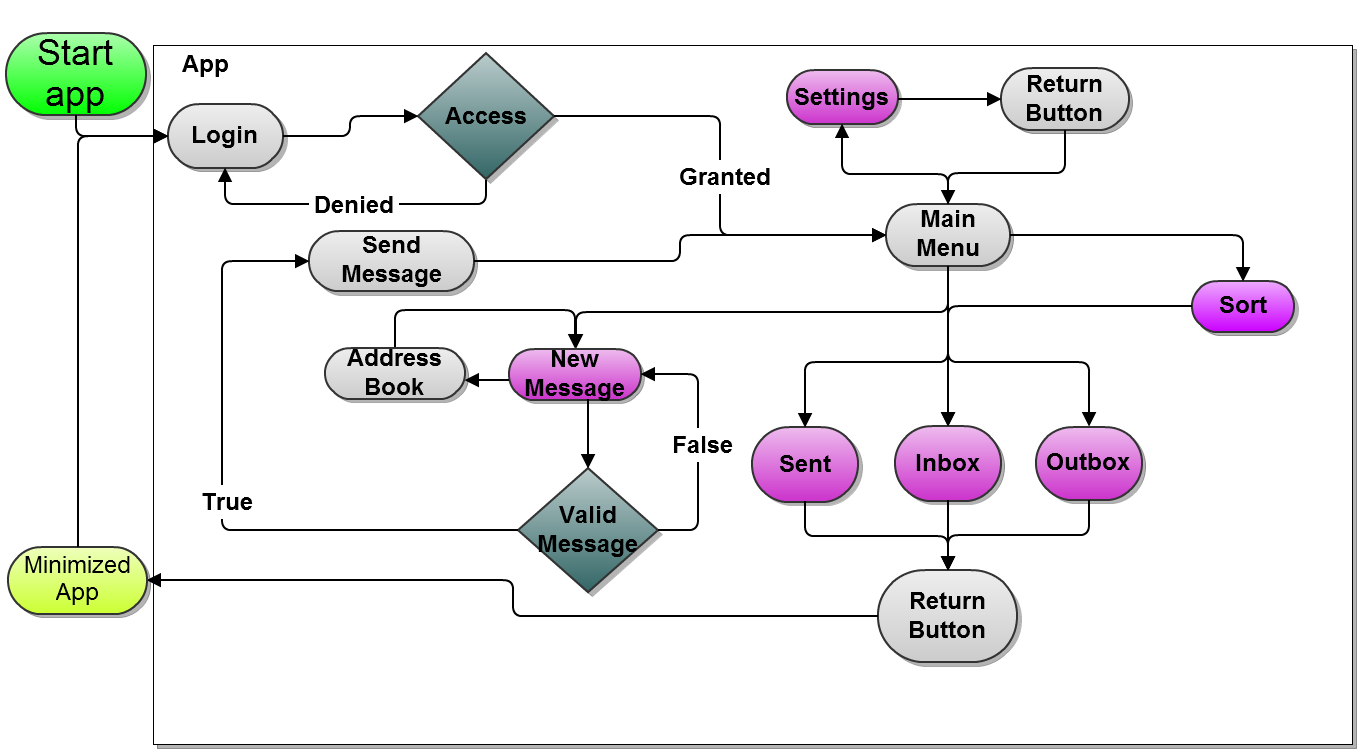
\includegraphics[width=\textwidth]{Android_GUI_flow_chart_2}
	\caption{The logical view of the GUI architecture}
	\label{fig:logicalGUIview}
\end{figure}

\subsubsection{Introduction}
The Android platform specifies a certain way of organizing the application, which we have tried to follow.

\subsubsection{External resources}
The user interface elements, ranging from whole screens (called layouts) to the structure and look of a single list element, are defined in \gls{xml} (Extensible Markup Language) and stored external to the application. An Android project contains a folder named “res” where all external resources are placed. User interface elements are stored in a sub folder called “layouts”. Other resources, e.g. colors or images, are stored inside separate sub folders. The advantage of declaring the user interface and other resources in \gls{xml} is that it enables decoupling of the presentation of the application and the code that controls the application.
\newline
\newline
All resources must be assigned an \gls{id} if they are to be referenced in the application code. All resource \gls{id}s are defined as public constants in the project’s R.class, which is a class that is automatically generated during build and contains subclasses for the types of resources where we have defined at least one resource, e.g. R.layout (for user interface elements) or R.color (for definition of colors). The resources can be referenced both inside other resources and in the application code.
\newline
\newline
We also want to use styles, which are collections of properties specifying the look of a layout or a component. It can be compared to the mindset of \gls{css}, where one separate design and content. We might also consider using a theme for our application, which is a style applied to an entire activity or application. The reason behind using styles and themes would be to ensure consistent appearance across the application. 

\subsubsection{Activities}
Activities are components that provide a screen that the user can interact with, and are classes written in Java. Each activity has a window where the user interface is drawn. One activity is specified as the main activity and is the start screen of the application. Each activity can start another activity to perform different actions. The activities inflate the \gls{xml} layouts to form the user interface and controls the behaviour of the elements. It is also possible to create layout elements programmatically, but we have chosen not to do this as we want the decoupling mentioned above.
\newline
\newline
An activity is always in one of four possible states \cite{bib:aas}:
\begin{itemize}
\item{}Active/running: When the activity is in the foreground of the screen
\item{}Paused: When the activity has lost focus but is still visible
\item{}Stopped: When the activity is completely obscured by another activity
\item{}If an activity is paused or stopped, it is likely that the system asks the activity to finish or just kill its process, hence drops it from memory. It then has to be restarted completely.
\end{itemize}

The life cycle of an activity can be seen in figure \ref{fig:lifecycle} at page \pageref{fig:lifecycle}.
\begin{figure}
	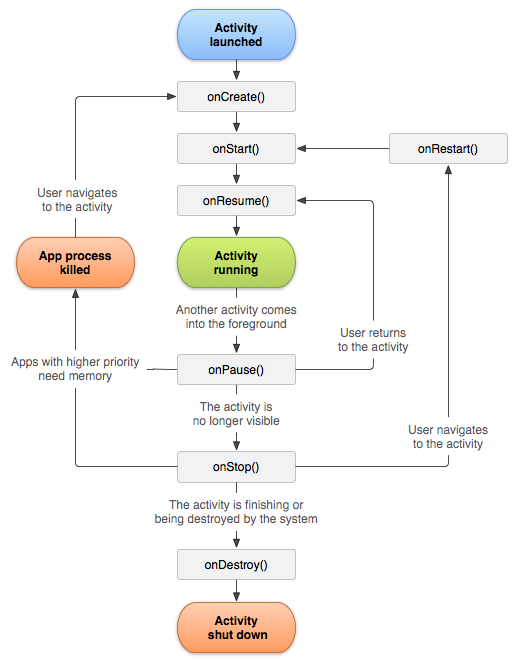
\includegraphics[width=\textwidth]{activity_lifecycle}
	\caption{Activity life cycle \cite{bib:alc}}
	\label{fig:lifecycle}
\end{figure}

All the methods starting with on (onCreate etc.) can be overwritten to administrate what the application should do in the changes of state.

\subsubsection{The Android manifest}
The Android manifest \cite{bib:aman} is what binds the applicaiton together. It is defined in \gls{xml} and details the structure and metadata of the application, its components and requirements. The manifest needs to have nodes for each of the components, which in our case are activities and services. Relevant metadata is the application name, icon and theme. The manifest also declares the permissions the application needs to access protected parts of the \gls{api} and interact with other applications.

\subsubsection{Supporting different hardware and internationalization}
By conforming to using external resources on can easily build applications that support differences such as varying screen sizes and languages. For example, it is possible to create a low, medium and high dpi (dots per inch, a measure of screen density) version of an image and Android will select the correct version based on the screen size. Android can pick layouts based on the screen orientation, where the possibilities are that the phone is an portrait or landscape mode. It is also possible to have Android decide what language to use based on location, but this is not relevant to this project. 